\documentclass[12pt,a4paper,oneside]{article}

\usepackage[utf8]{inputenc}
\usepackage[portuguese]{babel}
\usepackage[T1]{fontenc}
\usepackage{amsmath}
\usepackage{amsfonts}
\usepackage{amssymb}
\usepackage{graphicx}

\usepackage{xcolor}
% Definindo novas cores
\definecolor{verde}{rgb}{0.25,0.5,0.35}
\definecolor{jpurple}{rgb}{0.5,0,0.35}
% Configurando layout para mostrar codigos Java
\usepackage{listings}
\lstset{
  language=Java,
  basicstyle=\ttfamily\small, 
  keywordstyle=\color{jpurple}\bfseries,
  stringstyle=\color{red},
  commentstyle=\color{verde},
  morecomment=[s][\color{blue}]{/**}{*/},
  extendedchars=true, 
  showspaces=false, 
  showstringspaces=false, 
  numbers=left,
  numberstyle=\tiny,
  breaklines=true, 
  backgroundcolor=\color{cyan!10}, 
  breakautoindent=true, 
  captionpos=b,
  xleftmargin=0pt,
  tabsize=4,
  escapeinside=||
}

\author{\\Universidade Federal de Goiás (UFG) - Regional Jataí\\Bacharelado em Ciência da Computação \\Teoria dos Grafos \\Esdras Lins Bispo Jr.}

\title{\sc \huge Primeiro Teste}

\date{16 de maio de 2016}

\begin{document}

\maketitle

{\bf ORIENTAÇÕES PARA A RESOLUÇÃO}

\footnotesize

\begin{itemize}
	\item A avaliação é individual, sem consulta;
	\item A pontuação máxima desta avaliação é 10,0 (dez) pontos, sendo uma das 05 (cinco) componentes que formarão a média final da disciplina: dois testes, duas provas e exercícios;
	\item A média final ($MF$) será calculada assim como se segue
	\begin{eqnarray}
		MF & = & MIN(10, S) \nonumber \\
		S & = & 0,2.T_1 + 0,1.T_2 + 0,4.P_1 + 0,3.P_2 + E \nonumber
	\end{eqnarray}
	em que 
	\begin{itemize}
		\item $S$ é o somatório da pontuação de todas as avaliações,
		\item $T_i$ é a pontuação obtida no teste $i$,
		\item $P_i$ é a pontuação obtida na prova $i$, e
		\item $E$ é a pontuação total dos exercícios.
	\end{itemize}
	\item O somatório da pontuação de todas as questões desta avaliação é 11,0 (onze) pontos. Isto é um sinônimo de tolerância na correção. Se você por acaso perder 1,5 (um e meio), sua nota será 9,5 (nove e meio);
	\item O conteúdo exigido compreende os seguintes pontos apresentados no Plano de Ensino da disciplina: (1) Noções Básicas de Grafos e (2) Caminhos e Circuitos.
\end{itemize}

\begin{center}
	\fbox{\large Nome: \hspace{10cm}}
	\fbox{\large Assinatura: \hspace{9cm}}
\end{center}

\newpage

\normalsize

\begin{enumerate}

	\item (5,0 pt) De acordo com o vídeo do Prof. Paulo Cezar, apresente uma justificativa para que o grafo abaixo não possa ter um circuito euleriano?
	\begin{center}
	    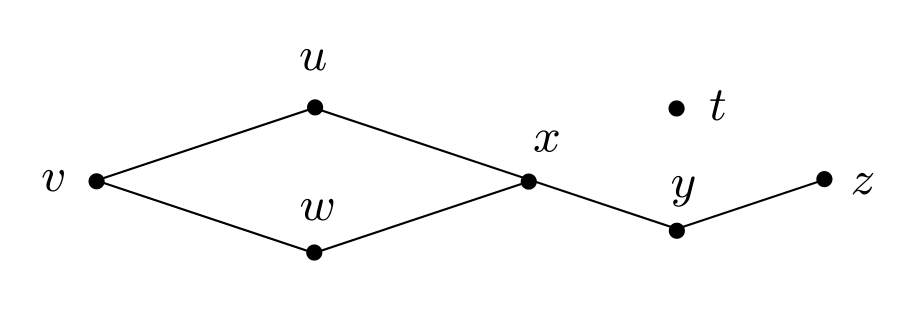
\includegraphics[width=10cm]{images/grafo.png}
	\end{center}
	
	{\color{blue} {\bf Resposta:} De acordo com o Prof. Paulo Cezar, um grafo conexo tem um circuito hamiltoniano se, e somente se, todos os vértices deste grafo têm grau par. Este grafo não pode ter um circuito euleriano porque o vértice $x$ tem grau ímpar. Pois, para se formar o circuito euleriano, quando se passa por $x$, necessariamente é preciso ``sair'' de $x$. Desta forma, a quantidade de entradas tem que ser igual a quantidade de saídas, forçando que ``arestas de entrada'' e ``arestas de saída'' estejam aos pares. Logo, o grau de todos os vértices tem que ser par. }
	
	\newpage
	
	\item (5,0 pt) [E 1.6] Seja $V$ o produto cartesiano $\{1,2, \ldots, p\} \times \{1,2, \ldots, q\}$, isto é, o conjunto de todos os pares ordenados $(i,j)$ em que $i \in \{1, \ldots, p\}$ e  $j \in \{1, \ldots, q\}$. Dizemos que dois elementos $(i,j)$ e $(i',j')$ são adjacentes se 
	\begin{center}
	    $i = i'$ e $|j - j'|=1$ \\
	    ou \\
	    $j = j'$ e $|i - i'|=1$
	\end{center}
	Essa relação de adjacência define um grafo sobre o conjunto $V$ de vértices. Esse grafo é conhecido como grade $p$-por-$q$. Quantas arestas tem a grade $p$-por-$q$?
	
	{\color{blue} {\bf Resposta:} Podemos calcular as arestas de uma grade $p$-por-$q$ em duas partes. Primeiro, calcularemos todas as arestas que formam as colunas. Segundo, calcularemos todas as arestas que formam as linhas. 
	
	Cada coluna tem $p-1$ arestas, pois entre duas linhas, sempre há uma aresta. Como se tem $q$ linhas, então temos $(p-1)q$ arestas que formam colunas.
	
	Cada linha tem $q-1$ arestas, pois entre duas colunas, sempre há uma aresta. Como se tem $p$ colunas, então temos $(q-1)p$ arestas que formam linhas.
	
	Logo, a quantidade de arestas de uma grade $p$-por-$q$ é a soma da quantidade de arestas que formam as linhas e a quantidade de arestas que formam as colunas. A quantidade de arestas de uma grade $p$-por-$q$  é $(p-1)q + (q-1)p$.}
	
	\end{enumerate}
\end{document}